% Name: Production possibility frontier
% Description: The bowed-out frontier of what an economy can make of two goods: an efficient point on it, a wasteful one inside, and one out of reach.
% Tags: production possibility frontier, opportunity cost, efficiency, scarcity

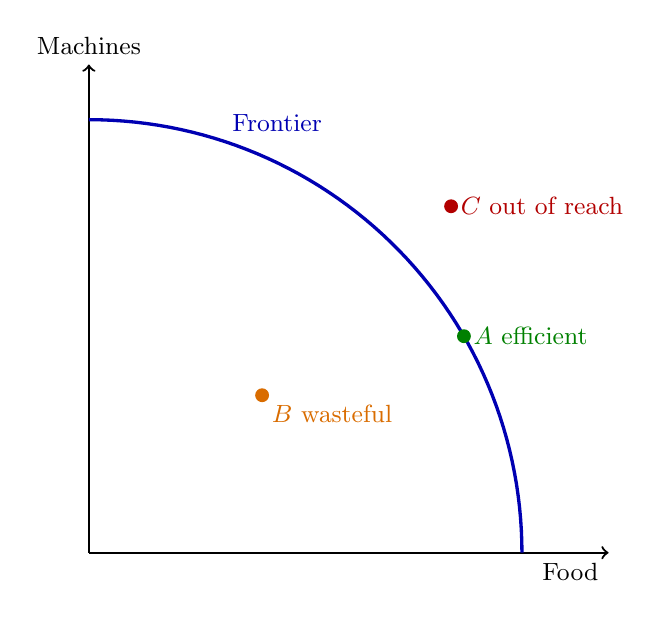
\begin{tikzpicture}[every node/.style={font=\small}]
  \draw[->, thick] (0,0) -- (6.6,0) node[below left] {Food};
  \draw[->, thick] (0,0) -- (0,6.2) node[above] {Machines};
  \draw[very thick, blue!70!black, domain=0:90, samples=60] plot ({5.5*cos(\x)}, {5.5*sin(\x)});
  \node[blue!70!black, above right] at (72:5.5) {Frontier};
  \fill[green!50!black] (30:5.5) circle (2.5pt) node[right] {$A$ efficient};
  \fill[orange!85!black] (2.2,2) circle (2.5pt) node[below right] {$B$ wasteful};
  \fill[red!70!black] (4.6,4.4) circle (2.5pt) node[right] {$C$ out of reach};
\end{tikzpicture}
